\newpage
\section{Concepts for Implementation}\label{sec:concepts}
In the previous chapters we discussed some possible security concepts and extensions for the Service Location Protocol (SLP). In the following sections we offer solutions to fulfill the requested requirements.\\
First of all we need to establish security groups, where users can communicate with authentications, using encryption and having message integrity. To create those groups we combined the already implemented SLP scopes with a group key agreement protocol (GKA). For this purpose we took the Tree-based Group Diffie-Hellman protocol (TGDH) to create and share security group keys (details about TGDH will be introduced in section \ref{sec:TGDH}). We will argue why we picked this protocol and how we integrated it into the SLP in detail.\\
Further we will discuss possible attacks on SLP which uses TGDH offer solutions we made for prevention.

\subsection{Security Groups}
As discussed earlier we propose to create security groups in an open network to establish security and still offer all SLP functions. To create a secured group within an open network we worked out a concept for a new workflow for our SecuredSLP. First of all a security group in SecuredSLP is a SLP scope in which the group members use encryption to communicate with each other. That means the group members all share a secret. To create and share a secret we use the TGDH protocol. The most important requirements to a security group are:
\begin{itemize}
  \item A plain text message, containing the name and the acces, should inform about a secured group and enable new users to join it.
  \item After a user is allowed to join a group, he requires the shared secret of this group, the group key (see also sections \ref{sec:TGDH} and \ref{sec:keyexchange}). This key could be a manual distributed pre-shared key (e.g. an administrator provides network members with a group key) or a automatic generated and distributed key (e.g. a group key agreement protocol which generates and distributes the group key)
  \item With a valid group key the user can decrypt all announced service information or offer services himself.
  \item If a user leaves a secured group, the secured group key should be refreshed automatically.
\end{itemize}
We choose TGDH because it fulfills all the requirements above and we already found an implementation in java for it. But it is not necessary to use TGDH, any other group key agreement protocol would work as well.\\
With TGDH each user within a security group has several cryptographic keys which are important for the communication with other members.\\
\textbf{Group Shared Key (GSK):} This key is equal for all group members and allows to access the secured group.\\
\textbf{Private-/Public-Key:} This is a key-pair every user uses to sign or verify the messages.

\subsection{Tree-based Group Diffie-Hellman (TGDH)}\label{sec:TGDH}
Tree-based Group Diffie-Hellman (TDHG) is a protocol-suite for group key management. It manages the key distribution between all network members. TGDH is based on a binary tree structure. But the tree structure is only logical which means it is not connected with the real positions of the network members. This protocol-suite handles several dynamic group events, for example new joinings or exits, fusions of networks and network partition. So TGDH implements four messages: \textsl{join}, \textsl{leave}, \textsl{merge} and \textsl{partition}\footnote{The merge and partition messages are extensions of the join and leave messages so we won't discuss them in this paper in detail. For more information about TGDH and their messages see also \citep{Liao2004}}. But all of these messages have some common structures within the following features:
\begin{itemize}
  \item Each network member computes the \textsl{group session key} out of the \textsl{group key} with a hash-function (the hash-function is the same for all members).
  \item Each \textsl{member session key} is just known to one member and should not be published.
  \item In case a group gets larger, the \textsl{session keys} of new members will be included and some of old members have to refresh their \textsl{session key}.
  \item In case a group gets smaller, the \textsl{session keys} of the members, who left the group, will be deleted and at least one member of the group refreshes his \textsl{session key}.
  \item All protocol-messages are signed by the sender. For the digital signature TGDH uses RSA or DSA with SHA-1 hash-function. 
\end{itemize}
After any changes each member refreshes his \textsl{key-tree} independently from each other. At this point the network quality and the device performance are very important. The group shared key itself isn't distributed but need to be calculated by each network peer himself. Only after receiving all information from the sponsor the peers are able to compute the group shared key \citep{Liao2004}.\\

\subsubsection{Keys in TGDH}
There are several cryptographic keys which are used in TGDH \citep{Liao2004}.
\begin{description}
\item[Group key] $K_{<0,0>}$ which is represented as the root of the TGDH tree (compare with figure \ref{fig:tgdh_tree}).
\item[Group session key] $K_{\text{\textit{group}}}$ which is derived from the group key. $K_{\text{\textit{group}}} = h(K_{<0,0>})$, where $h()$ is a cryptographic hash-function.
\item[Member session key] $K_i$ is a session key for the member $M_i$. 
\item[Blinded key] $BK_i$ is a key which can be calculated from the member session key $K_i$ with the function $BK_i = f(K_i)$, where $f() = g^k~mod~p$ with $g$ as generator and $p$ as a prime.
\end{description}
Furthermore there are also key sets the members have knowledge about. Each member knows all keys and their corresponding blinded keys in his path from the leaf to the root in the tree. For example member $M_2$ in the figure \ref{fig:tgdh_tree} knows the set of keys $\{K_{<2,1>}, K_{<1,0>}, K_{<0,0>}\}$ and the set of blinded keys $\{BK_{<2,1>}, BK_{<1,0>}, BK_{<0,0>}\}$. This information enalbles you aswell to compute any other key:
\begin{align*}
K_{<l,v>} &= (BK_{<l+1, 2v+1>})^{K_{<l+1, 2v>}}~mod~p\\
&= (BK_{<l+1, 2v>})^{K_{<l+1, 2v+1>}}~mod~p\\
&= g^{K_{<l+1, 2v>}K_{<l+1, 2v+1>}}~mod~p\\
&= f(K_{<l+1, 2v>}K_{<l+1, 2v+1>})
\end{align*}
It is also possible to compute the group key out of that information. For member $M_2$ the calculation would be:
\begin{align*}
K_{<0,0>} &= (BK_{<1,1>})^{K_{<1,0>}}~mod~p\\
&= (BK_{<1,1>})^{(BK_{<2,1>})^{K_{<2,0>}}}~mod~p
\end{align*}
\begin{figure}[!h]
\centering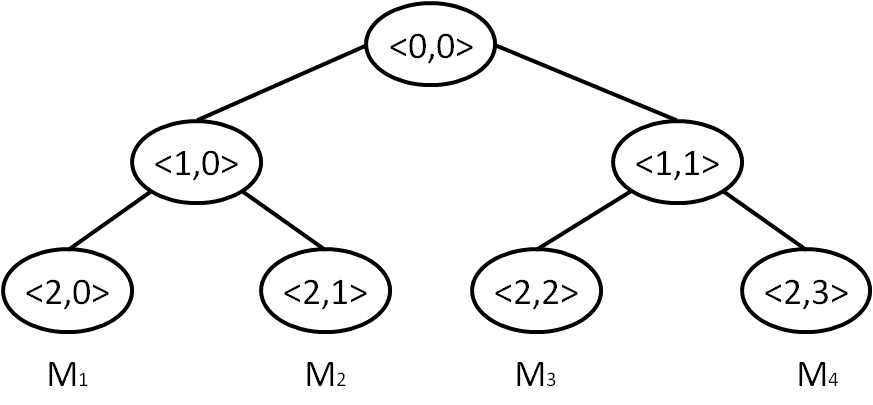
\includegraphics[width=0.4\textwidth]{Images/tgdh_tree}
\caption{Example of a tree structure in TGDH}
\label{fig:tgdh_tree}
\end{figure}

\subsubsection{Join message}
Assume a group with three members $\{M_1, M_2, M_3\}$ and a fourth user $M_4$ who wants to join this group. $M_4$ initializes the joining by sending a \textit{JoinMessage} to the group via multicast. The message contains the blinded key of $M_4$. First of all the join position for $M_4$ is calculated and a \textit{sponsor} is chose. The sponsor is the member whose leaf is placed on the insert position of the new member. In this case all members insert a new joint and a new leaf in their tree and delete all blinded keys in the path of the sponsor. Additionally the sponsor generates the new group session key and all keys and blinded keys in his path. Finally the sponsor sends the new tree $\widehat{T}$ and a set of all blinded keys via a multicast message. Member $M_1$ and $M_2$ can just calculate the group key after they received the new tree $\widehat{T}$. The tree update is shown in figure \ref{fig:tgdh_join}.
\begin{figure}[!h]
\centering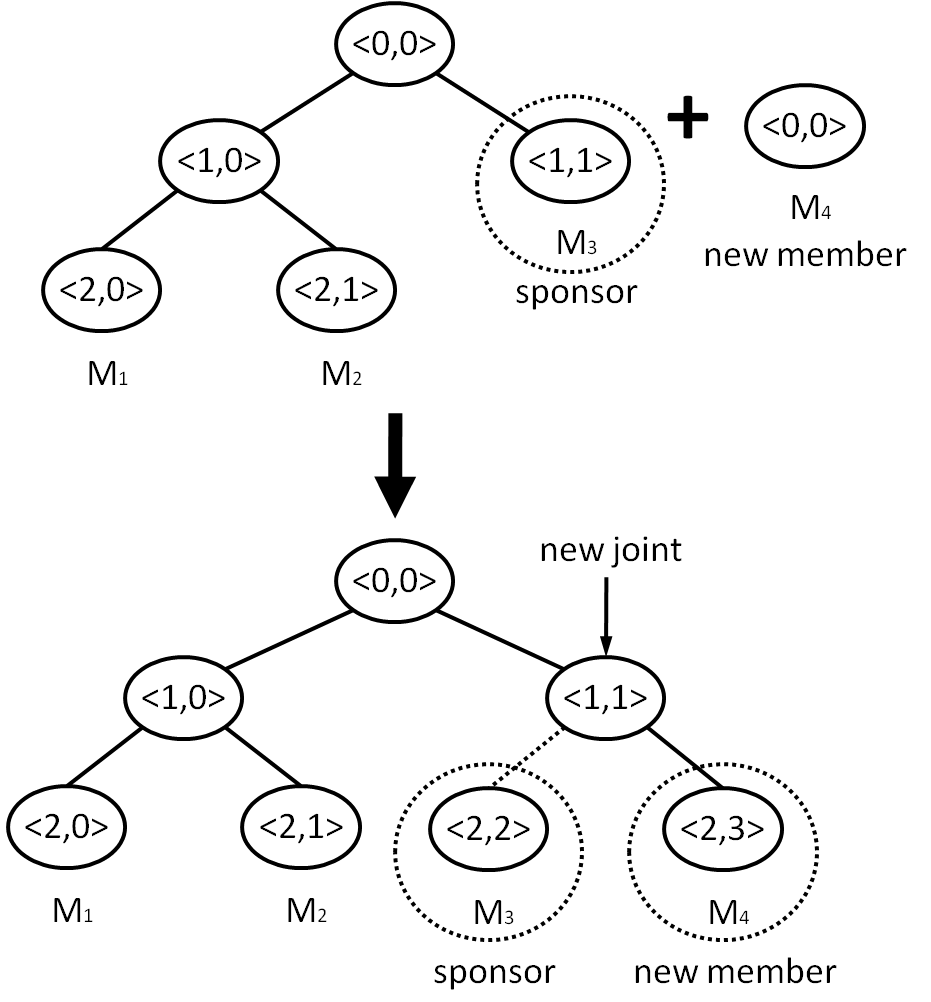
\includegraphics[width=0.5\textwidth]{Images/tgdh_join}
\caption{Tree update after a join of a new member}
\label{fig:tgdh_join}
\end{figure}

\subsubsection{Leave message}
To leave the group a member sends a \textit{LeaveMessage} via multicast to the group. Same as in \textit{JoinMessage}, a sponsor is chosen. All members remove the leaf and his father joint from the tree. They also remove all keys and blinded keys in the corresponding path. Additionally the sponsor generates new session keys and computes all keys and blinded keys in his path. In the end sponsor sends the new tree $\widehat{T}$ and a set of all blinded keys via broadcast to the group. After receiving the new tree, all other members are able to compute the new group key. The corresponding tree is illustrated in figure \ref{fig:tgdh_leave}.
\begin{figure}[!h]
\centering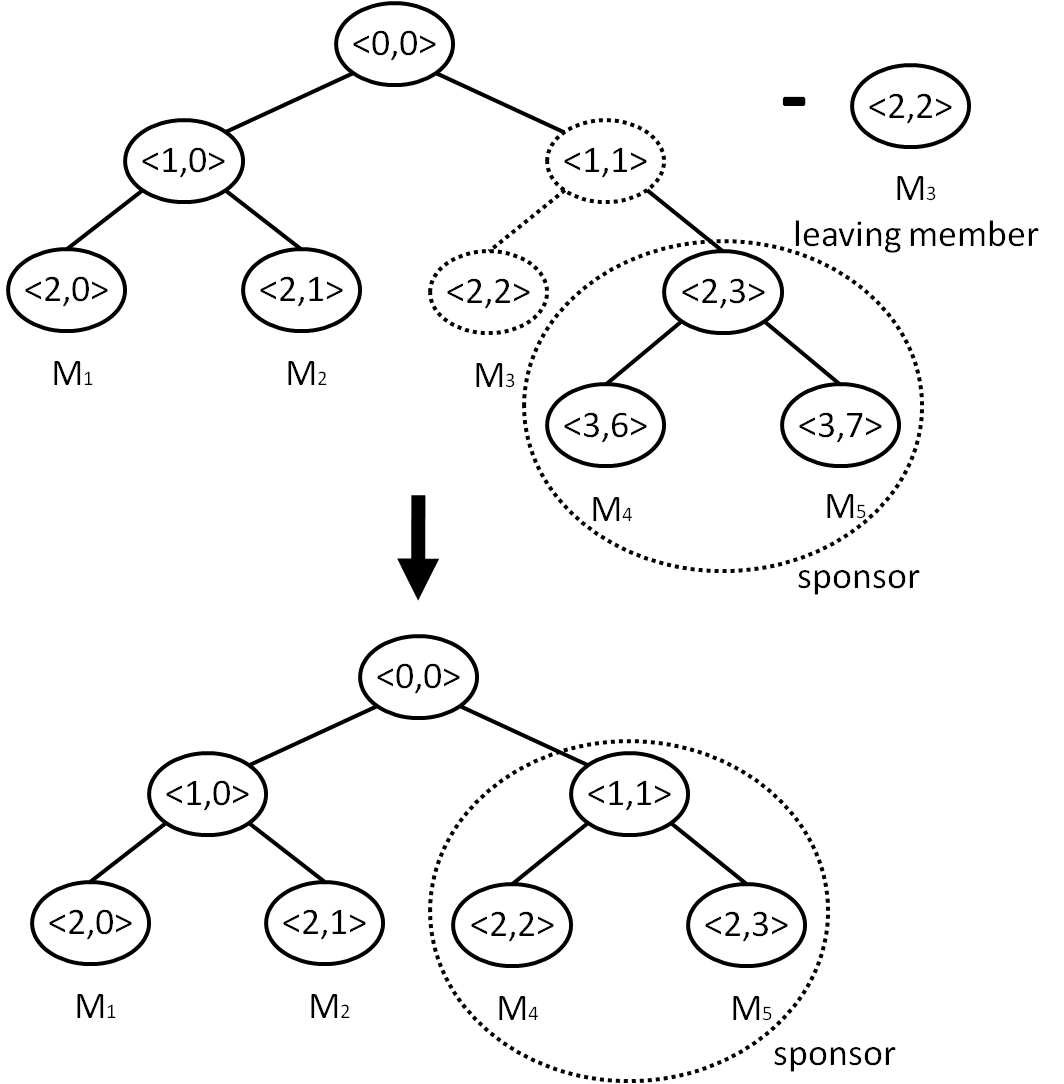
\includegraphics[width=0.5\textwidth]{Images/tgdh_leave}
\caption{Tree update after a member left the group}
\label{fig:tgdh_leave}
\end{figure}\noindent